\section{The universal factor $\cosh(au)$ and the clock}\label{pol:sec:cosh}

Multiplying the kernel by $e^{au}$ is an Esscher tilt of the P\'olya density and moves the basepoint: $\int_{-\infty}^{\infty}\Phi(u)e^{au}\cosh(wu)\,du=\frac12\left(\xi(\tfrac12+a+w)+\xi(\tfrac12+a-w)\right)$. The tilt alone destroys evenness. P\'olya's universal factor $\cosh(au)$ is the even average of the two tilts. Define, for $a\ge0$ and $\alpha=1/2+a$,
\begin{equation}\label{pol:eq:A}
A_\alpha(w)=2\int_0^\infty\Phi(u)\cosh(au)\cosh(wu)\,du=\tfrac12\left(\xi(\alpha+w)+\xi(\alpha-w)\right),
\end{equation}
the even part in $w$ of the basepoint function $w\mapsto\xi(\alpha+w)$. For real $t$, $A_\alpha(it)=\re\xi(\alpha+it)$, and in the variable $s=1/2+w$ this is Lagarias's function $A_h(s)=\frac12(\xi(s+h)+\xi(s-h))$ with $h=a$.

\begin{theorem}[P\'olya, de Bruijn, Lagarias]\label{pol:thm:cosh}
\begin{enumerate}
\item[(i)] Under RH, $A_\alpha$ has only purely imaginary zeros for every $\alpha>1/2$.
\item[(ii)] If every zero of $\Xi$ satisfies $|\im t|\le\Delta$, then every zero of $t\mapsto A_\alpha(it)$ satisfies $|\im t|\le\max(\Delta^2-a^2,0)^{1/2}$. In particular, unconditionally, $A_\alpha$ has only purely imaginary zeros for $\alpha\ge1$, and they are simple.
\item[(iii)] If $A_{\alpha_n}$ has only imaginary zeros along a sequence $\alpha_n\downarrow1/2$, then RH holds.
\end{enumerate}
\end{theorem}

\begin{proof}
(i) $\cosh(au)$ is a universal factor since $\cos(az)\in\mathcal{LP}$. (ii) is de Bruijn's strip theorem for the factor $\cosh$, and $\Delta\le1/2$ because $\zeta$ has no zeros with $\re s>1$; simplicity is Lagarias's theorem \cite{Lagarias05}. (iii) $A_\alpha\to\xi(1/2+w)$ locally uniformly as $\alpha\downarrow1/2$, and Hurwitz's theorem applies.
\end{proof}

\begin{corollary}[Even part basepoint laws]\label{pol:cor:evenpart}
Whenever $A_\alpha$ has only imaginary zeros $\pm i\tau_k$, the function $\varphi^P_\alpha(s)=\xi(\alpha)/A_\alpha(\sqrt s)$ is the Laplace transform of a GGC law $\mu^P_\alpha$ with Thorin measure $\sum_k\delta_{\tau_k^2}$, so $\mu^P_\alpha$ is the law of $\sum_kE_k/\tau_k^2$. This holds unconditionally for $\alpha\ge1$, for all $\alpha>1/2$ under RH, and RH follows if it holds along a sequence $\alpha_n\downarrow1/2$.
\end{corollary}

\begin{proof}
$A_\alpha(\sqrt s)$ is entire of order one half in $s$ with positive Taylor coefficients by \eqref{pol:eq:A}, value $\xi(\alpha)>0$ at $s=0$, and zeros $s=-\tau_k^2$; the genus zero product gives $\varphi^P_\alpha(s)=\prod_k(1+s/\tau_k^2)^{-1}$.
\end{proof}

\begin{proposition}[Half integer crossings]\label{pol:prop:round}
Let $\alpha$ be such that $\xi$ has no zeros in $\re s\ge\alpha$ (this holds for $\alpha>\sigma_{\max}$, and unconditionally for every $\alpha\ge1$, since $\zeta$ has no zeros on $\re s=1$). Then the clock $U_\alpha$ is continuous and strictly increasing from $U_\alpha(0)=0$, and the positive zeros of $t\mapsto\re\xi(\alpha+it)$ are exactly
\begin{equation}\label{pol:eq:quantile}
\tau_k=\tau_\alpha\!\left(k-\tfrac12\right),\qquad k=1,2,\dots,
\end{equation}
where $\tau_\alpha$ is the inverse of the clock. Consequently the Thorin distribution of the even part law is the rounding of the Thorin distribution of the basepoint law,
\begin{equation}\label{pol:eq:round}
U^P_\alpha\big((0,T^2]\big)=\left\lfloor U_\alpha(T)+\tfrac12\right\rfloor,
\end{equation}
and in law $\mu^P_\alpha=\mathcal L\big(\sum_kE_k/\tau_\alpha(k-\tfrac12)^2\big)$ while $\mu^{(\alpha)}=\mathcal L\big(\int_0^\infty dg_v/\tau_\alpha(v)^2\big)$: the even part law is the midpoint rule for the gamma clock integral.
\end{proposition}

\begin{proof}
Since no zero has $\beta_\rho\ge\alpha$, the Hadamard sum $\re\frac{\xi'}{\xi}(\alpha+i\tau)=\sum_\rho\frac{\alpha-\beta_\rho}{|\alpha+i\tau-\rho|^2}$ has every term positive, so the clock is strictly increasing, and $\xi(\alpha+i\tau)\ne0$. Write $\xi(\alpha+i\tau)=|\xi(\alpha+i\tau)|e^{i\pi U_\alpha(\tau)}$, which is legitimate since $\xi(\alpha)>0$. Then $\re\xi(\alpha+i\tau)=|\xi(\alpha+i\tau)|\cos(\pi U_\alpha(\tau))$ vanishes exactly when $U_\alpha(\tau)\in\mathbb Z+\frac12$, and a strictly increasing clock starting at $0$ and tending to infinity (by Stirling, $U_\alpha(\tau)\sim\frac\tau{2\pi}\log\tau$) crosses each level $k-\frac12$ exactly once, transversally. This gives \eqref{pol:eq:quantile} and simple zeros. Every zero $\rho$ has $|\beta_\rho-\frac12|<\alpha-\frac12$, by the hypothesis and the functional equation, so Theorem~\ref{pol:thm:cosh}(ii) with $\Delta=\alpha-\frac12$ shows that $A_\alpha$ has no zeros off the imaginary axis, and the corollary on even part laws applies; counting levels below $U_\alpha(T)$ then gives \eqref{pol:eq:round}. The two laws follow from the gamma process representation: the increments of $g$ over $[k-1,k]$ are independent standard exponentials, and replacing $\tau_\alpha(v)$ on $[k-1,k]$ by its midpoint value gives the sum.
\end{proof}

Under the hypothesis of Proposition~\ref{pol:prop:round}, which holds unconditionally for $h\ge\frac12$ and under RH for every $h>0$, the proposition explains why the zeros of $A_h$ are asymptotically equally spaced, as in Lagarias's theorem \cite{Lagarias05}: they are level crossings of a smooth increasing clock whose derivative $\pi^{-1}\re\xi'/\xi(\alpha+i\tau)$ is a Cauchy smoothing of the zero density, with fluctuations of lower order than its mean $\frac1{2\pi}\log\frac\tau{2\pi}$.

\paragraph{Numerics.} Table~\ref{pol:tab:clock} lists, for four basepoints, the number of zeros of $\re\xi(\alpha+it)$ on $(0,100]$, the clock at $100$, its rounding, and the largest distance of the clock from a half integer at the computed zeros (on a grid of step $0.01$ with linear interpolation). As $\alpha\downarrow1/2$ the atoms converge to the ordinates.

\begin{table}[ht]
\centering\small
\fitwidth{\begin{tabular}{ccccc}
\toprule
$\alpha$ & zeros on $(0,100]$ & $U_\alpha(100)$ & $\lfloor U_\alpha(100)+\frac12\rfloor$ & $\max$ distance to $\mathbb Z+\frac12$\\
\midrule
$1.00$ & 29 & 29.1112 & 29 & $2.7\times10^{-5}$\\
$0.75$ & 29 & 29.0548 & 29 & $5.6\times10^{-5}$\\
$0.60$ & 29 & 29.0218 & 29 & $1.7\times10^{-4}$\\
$0.52$ & 29 & 29.0044 & 29 & $1.6\times10^{-3}$\\
\bottomrule
\end{tabular}}
\caption{Atoms of the even part law against the rounded clock of the basepoint law.}\label{pol:tab:clock}
\end{table}

\begin{remark}[Is the P\'olya family easier?]\label{pol:rem:easier}
Real rootedness of $A_\alpha$ is a counting condition: it can be certified to a given height by sign changes of $\re\xi(\alpha+it)$ together with an argument principle count, exactly as in Turing's method. So the P\'olya family is not easier in principle, but it converts the analytic positivity of $\re\xi'/\xi$ into a discrete, verifiable statement about atoms. The zero trajectories $\alpha\mapsto\tau_k(\alpha)$ satisfy $d\tau_k/d\alpha=\re\xi'(s)/\im\xi'(s)$ at $s=\alpha+i\tau_k$. Under RH no two trajectories collide for $\alpha>\frac12$, because the zeros are simple (Proposition~\ref{pol:prop:round}); conversely a nonimaginary zero of $A_\alpha$ can appear only through a collision of two imaginary zeros, provided no zeros enter from infinity as $\alpha$ decreases, which needs uniform control of the zero counts in $\alpha$. In this heuristic sense RH is the statement that no two trajectories collide before $\alpha=\frac12$, a discrete analogue of the de Bruijn Newman dynamics.
\end{remark}

\section{P\'olya's $\Xi^*$ as the archimedean model}\label{pol:sec:xistar}

\begin{proposition}\label{pol:prop:bessel}
With \eqref{pol:eq:phistar},
\begin{equation}\label{pol:eq:bessel}
\Xi^*(t)=4\pi^2\left[K_{\frac94+\frac{it}2}(2\pi)+K_{\frac94-\frac{it}2}(2\pi)\right]=8\pi^2\re K_{\frac94+\frac{it}2}(2\pi).
\end{equation}
\end{proposition}

\begin{proof}
Substitute $v=2u$ in $2\int_0^\infty\Phi^*(u)\cos(tu)\,du$, write $\cosh(9v/4)\cos(tv/2)$ as the average of $\cos((t/2\mp9i/4)v)$, and use $\int_0^\infty e^{-a\cosh v}\cos(\omega v)\,dv=K_{i\omega}(a)$ and the evenness of $K_\nu$ in $\nu$.
\end{proof}

This is the identity of Section~\ref{ch:biane}, where $P(\theta)=K_{i\theta/2}(2\pi)$ and $\Xi^*(\theta)=4\pi^2[P(\theta-\frac{9i}2)+P(\theta+\frac{9i}2)]$.

Formula \eqref{pol:eq:bessel} says that $\Xi^*$ is exactly the construction \eqref{pol:eq:A} applied to the Bessel function: it is the even part, at basepoint $9/4$ in the order variable, of $\nu\mapsto K_\nu(2\pi)$. P\'olya's theorem that $K_{iz}(a)$ has only real zeros is the Riemann Hypothesis for this function: its zeros in $\nu$ lie on $\re\nu=0$. The basepoint $9/4$ lies strictly to the right of that line, so by the argument of Theorem~\ref{pol:thm:cosh} and Proposition~\ref{pol:prop:round} the even part has only real zeros (the argument needs $\re\frac d{d\nu}\log K_\nu(2\pi)>0$ on $\re\nu>0$, and this holds because $\nu\mapsto K_\nu(2\pi)$ is even, of order one, with only the zeros $\pm iz_n$, $z_n>0$, so that $K_\nu(2\pi)=K_0(2\pi)\prod_n(1+\nu^2/z_n^2)$ and each term $\frac{d}{d\nu}\log(1+\nu^2/z_n^2)=(\nu+iz_n)^{-1}+(\nu-iz_n)^{-1}$ has positive real part there), located where the Bessel clock $\pi^{-1}\arg K_{9/4+it/2}(2\pi)$ crosses half integers.

\begin{proposition}[Half Gram points]\label{pol:prop:gram}
Let $t_k^*$ be the positive zeros of $\Xi^*$ in increasing order and $\vartheta$ the Riemann Siegel theta function. Then\begin{equation}\label{pol:eq:gram}\frac{\vartheta(t_k^*)}{\pi}=k-\frac32-\frac{2\pi^2-3}{\pi\,t_k^*}+O\big((t_k^*)^{-2}\big).\end{equation} Hence, with $N^*(T)=\#\{k:t_k^*\le T\}$, $N^*(T)=\lfloor\vartheta(T)/\pi+\frac32\rfloor$ for all large $T$ outside the intervals $[t_k^*,t_k^*+O(1/(t_k^*\log t_k^*)))$, on which $N^*(T)$ is one larger; in particular $N^*(T)-\vartheta(T)/\pi$ is bounded, whereas $N(T)=\vartheta(T)/\pi+1+S(T)$.
\end{proposition}

\begin{proof}[Sketch]
For $\nu=\frac94+\frac{it}2$, the ascending series of $I_{-\nu}$ and the reflection formula give $K_\nu(2\pi)=\frac12\Gamma(\nu)\pi^{-\nu}\big(1+\frac{\pi^2}{1-\nu}+O(t^{-2})\big)$, the companion term $\frac12\Gamma(-\nu)\pi^\nu$ being smaller by a factor of order $t^{-9/2}$. With $s=\frac12+it$ we have $\Gamma(\nu)=(\frac s2+1)\frac s2\,\Gamma(\frac s2)$ and $\Gamma(\frac s2)\pi^{-it/2}=|\cdot|e^{i\vartheta(t)}$, so the phase of $K_\nu(2\pi)$ is $\vartheta(t)+\arg s+\arg(s+2)+\im\frac{\pi^2}{1-\nu}+O(t^{-2})$. Here $\arg s+\arg(s+2)=\pi-\frac3t+O(t^{-3})$ and $\im\frac{\pi^2}{1-\nu}=\frac{2\pi^2t}{t^2+25/4}=\frac{2\pi^2}{t}+O(t^{-3})$, so the phase is $\vartheta(t)+\pi+\frac{2\pi^2-3}{t}+O(t^{-2})$. The zeros of the real part are where this phase lies in $\frac\pi2+\pi\mathbb Z$, which is \eqref{pol:eq:gram}; the indexing is fixed by the first zero.
\end{proof}

Compare the Thorin form of the zero count, $U((0,t])=\vartheta(\sqrt t)/\pi+1+S(\sqrt t)$ under RH. P\'olya's $\Xi^*$ replaces the arithmetic fluctuation $S$ by a bounded rounding error: by Proposition~\ref{pol:prop:gram} its Thorin distribution $N^*(\sqrt t)$ is the rounding of the smooth archimedean distribution $\vartheta(\sqrt t)/\pi+1$. This is the distribution that the $2\sin^2$ lemma computes for the gamma factor in Theorem~\ref{rz:thm:gammaggc}, up to an affine function of $\sqrt t$: that theorem gives $(\vartheta(\sqrt t)-\vartheta'(0)\sqrt t)/\pi$ for the compensated factor $e^{-c\sqrt s}/G(s)$, with $c=-\vartheta'(0)$. In this sense $\Xi^*$ is the zeta function with $\zeta$ replaced by its first Dirichlet term and the result symmetrised, and its reciprocal $\Xi^*(0)/\Xi^*(\sqrt{-s})$ is, by P\'olya's theorem, an unconditional GGC with Thorin measure $\sum_k\delta_{(t_k^*)^2}$.

\paragraph{Numerics.} $\Xi^*$ has 29 zeros in $(0,100]$, as does $\Xi$, but they are displaced: the first eight are $8.9928$, $19.0654$, $24.4748$, $28.9750$, $33.0069$, $36.7367$, $40.2491$, $43.5947$. There are $138$ zeros up to height $300$; at the last, $t^*_{138}=299.627$, the deviation from $k-\frac32$ times $t^*_k$ is $-5.329$, against the constant $-(2\pi^2-3)/\pi=-5.328$ of \eqref{pol:eq:gram} (Figure~\ref{pol:fig:one}, right).

\begin{figure}[ht]
\centering
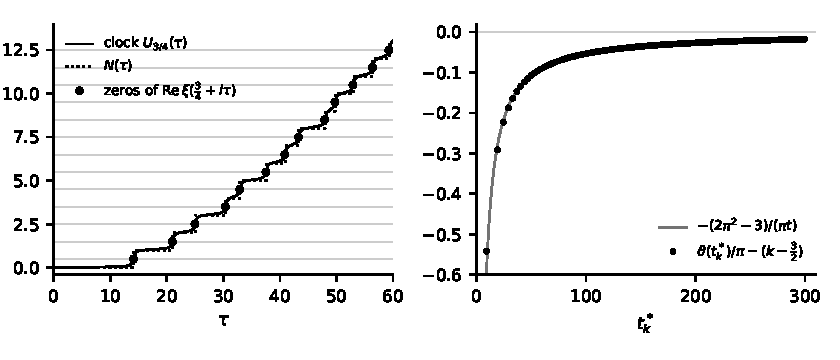
\includegraphics[width=\textwidth]{fig/polya_fig1.pdf}
\caption{Left: the clock $U_{3/4}(\tau)$ of the basepoint law at $\alpha=3/4$ for $0\le\tau\le60$, the zero count $N(\tau)$ (dotted), and the zeros of $\re\xi(3/4+i\tau)$, which sit exactly on the half integer levels (grey lines). Right: $\vartheta(t_k^*)/\pi-(k-\frac32)$ for the 138 zeros of P\'olya's $\Xi^*$ below height 300, with the asymptote $-(2\pi^2-3)/(\pi t)$ of Proposition~\ref{pol:prop:gram}.}\label{pol:fig:one}
\end{figure}

\section{P\'olya's Mellin criterion applied to the Riemann kernel}\label{pol:sec:mellin}

Take $q=1$ and $\mathcal F(v)=\Phi(\sqrt v)$ in P10, so that $\mathcal F(t^2)=\Phi(t)$ and the conclusion would be RH. The criterion asks that
\begin{equation}\label{pol:eq:M}
M(z)=\int_0^\infty\Phi(u)\,u^{2z-1}\,du=\tfrac12\int_0^\infty\mathcal F(v)v^{z-1}dv
\end{equation}
have no zeros in $\mathbb C\setminus(-\infty,0]$. The integral converges for $\re z>0$, and $M(k+\frac12)=\frac12(2k)!\,c_k>0$ and $2M(\frac12)=\xi(\frac12)$. Near the origin $\Phi(u)=\sum_{j\ge0}p_ju^{2j}$, with radius of convergence $\pi/4$, $p_0=\Phi(0)=0.893394$ and $p_1=-8.36525$; integrating termwise over $(0,\delta)$, $\delta<\pi/4$, gives $\int_0^\delta\Phi(u)u^{2z-1}du=\sum_jp_j\delta^{2z+2j}/(2z+2j)$, which continues $M$ to a meromorphic function with simple poles at $z=0,-1,-2,\dots$, and this continuation is the function that the criterion refers to.

The criterion does not apply to $\Phi$. If $X_\Phi$ has the P\'olya density $\Phi/\Xi(0)$ (the variable $X$ of Theorem~\ref{thm:ch13:mellin}, and not the $X$ of this chapter), then $\mathbb E|X_\Phi|^{2s}=2M(s+\frac12)/\Xi(0)$ with the $M$ of \eqref{pol:eq:M}, so that theorem says that $M$ has a simple zero at $z_1=s_1+\frac12=-7.99418226+2.93776707\,i$, which lies in $\mathbb C\setminus(-\infty,0]$. We checked this independently (\texttt{polya\_mellin\_z1.py}, at 60 digits, with two quadrature layouts): $|M|=8.0\times10^{-16}$ at the point $s_1+\frac12$ printed in that theorem, and on the circle $|z-z_1|=\frac12$ we have $|M|\ge0.224$ and the winding number of $M$ is $1$, so that $z_1$ is the only zero in the disc. So the hypothesis of the criterion fails for $q=1$. For $q\ge2$ the function $\mathcal F(t^{2q})$ has no $t^2$ term whenever $\mathcal F$ is holomorphic near the origin, whereas $\Phi(t)=0.893394-8.36525\,t^2+\cdots$, so there is no factorisation $\Phi(t)=\mathcal F(t^{2q})$ with $q\ge2$. The Mellin route of the 1927 paper is therefore closed for $\Phi$ itself, by the zero that closes the Bernstein Pick route in Theorem~\ref{thm:ch13:mellin}.

The zero $z_1$ is the only obstruction that we found. An argument principle scan of the continuation (\texttt{polya\_mellin.py}, floating point) finds no zero with $0.05\le|\im z|\le14.05$ in $-3.95\le\re z\le8.05$. A plain Gauss Legendre rule for \eqref{pol:eq:M} produces spurious zeros with $\re z<\frac12$, because the integrand has an integrable singularity $u^{2\re z-1}$ at the origin that oscillates like $\cos(2\im z\log u)$; the termwise integration on $(0,\frac14)$ removes the difficulty.
